\documentclass{beamer}
\usetheme{Madrid}
\usecolortheme{default}
\usepackage{tikz}
\usepackage{subfigure}

\title[]
{Efficient Hyperparameter Optimization of Deep Learning
Algorithms Using Deterministic RBF Surrogates}


\author[Yakovlev Konstantin]
{Yakovlev Konstantin}


\date[2023] % (optional)
{BMM, March 2023}


\definecolor{uoftblue}{RGB}{6,41,88}
\setbeamercolor{titlelike}{bg=uoftblue}
\setbeamerfont{title}{series=\bfseries}

\begin{document}

\frame{\titlepage}


\begin{frame}
\frametitle{Goals of the research}

\begin{block}{Problem}
  Automatically searching for optimal hyperparameter configurations
\end{block}

\begin{block}{Challenge}
  Probabilistic surrogates require accurate estimates of sufficient statistics.
  This makes them inefficient for optimizing hyperparameters of deep learning algorithms.
\end{block}

\begin{block}{Solution}
  Consider radial basis functions as error surrogates. The proposed algorithm
  (HORD) requires fewer function evaluations.
\end{block}

\end{frame}


\begin{frame}
  \frametitle{Problem statement}
  Geven a set of hyperparameters $\mathbb{R}^D$, train and validation datasets:
  $\mathfrak{D}_\text{train/val}$, model parameters $\boldsymbol{\theta}$, and
  black-box error function $f$.
  \begin{align*}
    \min_{\mathbf{x}\in \mathbb{R}^D}\quad &f(\mathbf{x}, \boldsymbol{\theta}, \mathfrak{D}_\text{val}), \\
    \mathrm{s.t.} \quad &\boldsymbol{\theta} = \arg\min_{\boldsymbol{\theta}}f(\mathbf{x}, \boldsymbol{\theta}, \mathfrak{D}_\text{train})
  \end{align*}
  
\end{frame}


\begin{frame}
  \frametitle{The Method}
  \textbf{The surrogate model}\\
  Given a hyperparameter configuration $\mathbf{x}_{1:n}$ of size $n$ and its corresponding
  validation errors $f_{1:n}$. Define the RBF interpolation model as:
  \[
    S_n(\mathbf{x}) = \sum_{i=1}^n\lambda_i\phi(\|\mathbf{x} - \mathbf{x}_i\|_2) + 
    p(\mathbf{x}),
  \]
  where $\phi(r) = r^3$ - cubic spline RBF, $p(\mathbf{x}) = \mathbf{b}^\top\mathbf{x} + a$.
  The parameters of the spline are determined by solving the following system:
  \[
  \begin{cases}
    \mathbf{\Phi}\boldsymbol{\lambda} + \mathbf{P}\mathbf{c} = \mathbf{F}, \quad
    \mathbf{\Phi} = \{\phi(\|\mathbf{x}_i - \mathbf{x}_j\|_2)\}_{i, j=1}^n,\;
    \mathbf{P} = [\{\mathbf{x}_i^\top, 1\}_{i=1}^n]^\top \\
    \mathbf{P}^\top\boldsymbol{\lambda} = \mathbf{0}, \quad \mathbf{F} = [\{f(\mathbf{x}_i)\}_{i=1}^n],\;
    \mathbf{c} = [\mathbf{b}, a].
  \end{cases}
  \]

\end{frame}


\begin{frame}
\frametitle{Spline theory}
% \begin{alertblock}{Theorem}
%   For any arbitrary non-zero $\boldsymbol{\lambda}: \sum_{i=1}^n\lambda_i q(\mathbf{x}_i) = 0$ for any
%   linear form $q$ the following is true:
%   \[
%     \boldsymbol\lambda^\top\mathbf{\Phi}\boldsymbol{\lambda} > 0.
%   \]
% \end{alertblock}
% \begin{block}{Remark}
%   Alternative condisions are $\mathbf{P}^\top\boldsymbol{\lambda} = \mathbf{0}$.
% \end{block}
% Now make sure that if $\mathbf{P}^\top\boldsymbol{\lambda} = 0$, then the spline minimizes
% an energy (suppose $\mathbf{x} \in \mathbb{R}$):
% \begin{align*}
%   J(S) = \int_{\mathbb{R}^1}[S''(\mathbf{x})]^2d\mathbf{x} = 12\sum_{i=1}^n\lambda_iS(\mathbf{x}_i)=
% 12\boldsymbol{\lambda}^\top\mathbf{\Phi}\boldsymbol{\lambda} > 0.
% \end{align*}
Show that $\mathbf{P}^\top\boldsymbol{\lambda} = \mathbf{0}$ is necessary for minimizing energy.
For simpicity, consider $D = 1$.
\begin{align*}
  J(S) = \int_{\mathbb{R}^1}[S''(\mathbf{x})]^2d\mathbf{x} = 12\sum_{i=1}^n\lambda_iS(\mathbf{x}_i)= \\
  12(\boldsymbol{\lambda}^\top\mathbf{\Phi}\boldsymbol{\lambda} + \boldsymbol{\lambda}^\top\mathbf{P}\mathbf{c})
  \to \min_{\mathbf{c}} \Rightarrow \mathbf{P}^\top\boldsymbol{\lambda} = \mathbf{0}.
\end{align*} 

\begin{alertblock}{Theorem}
  A matrix $\begin{pmatrix}\mathbf{\Phi} & \mathbf{P} \\ \mathbf{P}^\top & \mathbf{0}\end{pmatrix}$
  is non singular $\Leftrightarrow$ columns of $\mathbf{P}$ are linearly dependent.
  \footnote{See (2.11) of Gutmann, 2001}
  
\end{alertblock}

\end{frame}


\begin{frame}
  \frametitle{Latin hypercube sampling\footnote{https://artowen.su.domains/mc/Ch-var-adv.pdf}}
  % TODO: https://www.asc.ohio-state.edu/statistics/comp_exp/jour.club/McKayConoverBeckman.pdf
  \begin{minipage}{.3\textwidth}
  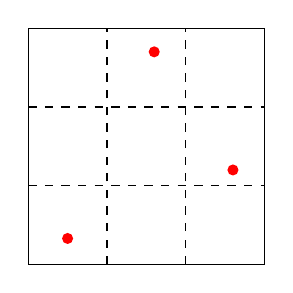
\begin{tikzpicture}
    \draw (0,0) -- (3,0) -- (3,3) -- (0,3) -- (0,0);
    \draw[dashed] (0,1) -- (3,1);
    \draw[dashed] (0,2) -- (3,2);
    \draw[dashed] (1,0) -- (1,3);
    \draw[dashed] (2,0) -- (2,3);
    \fill[red] (0.5,0.33) circle (2pt);
    \fill[red] (1.6,2.7) circle (2pt);
    \fill[red] (2.6,1.2) circle (2pt);
  \end{tikzpicture}
  \end{minipage}%
  \begin{minipage}{.7\textwidth}
  The task is to generate $n_0$ samples from $\mathbf{U}[0, 1]^D$. Let $U_{ij}$ be i.i.d. samples
  from $U[0, 1]$, and $\boldsymbol{\pi}$ is a uniform permutation of $\overline{0, n_0-1}$.
  Then
  \[
    X_{ij} := \frac{\pi_j(i - 1) + U_{ij}}{n_0}, \quad i = \overline{1, n_0}, \;
    j = \overline{1, D}. 
  \]
  \end{minipage}

  \begin{alertblock}{Theorem}
    Let $X_{ij}$ be a Litin hypercube samples. Then $\mathbf{X}_i \sim \mathbf{U}[0, 1]^D$
    for each $i = \overline{1, n_0}.$
  \end{alertblock}
\end{frame}


\begin{frame}
  \frametitle{General algorithm}
  \begin{enumerate}
    \item Start by drawing $n_0 = 2(D + 1)$ samples, using Latin hypercube sampling.
    \item While $n < N_\text{max}$, maximum evaluation number, generate $m = 100D$ candidates
    $\mathbf{t}_{n, 1:m}$. The probability of perturbing a coordinate:
    \[
      \varphi_n = \min(20/D, 1)\left[1 -\frac{\log(n - n_0 + 1)}{\log(N_\text{max} - n_0)}\right].
    \]
    The additive perturbation $\delta_i \sim \mathcal{N}(0, \sigma_n^2)$, where $\sigma_{n_0}^2 = 0.2$,
    after each $\max(5, D)$ iteration with no improvements
    $\sigma_{n+1}^2 = \min(\sigma_n^2/2, 0.005)$. After 3 consecutive iterations with improvement
    $\sigma_{n+1}^2 = \min(0.2, 2\sigma_n^2)$.
  \end{enumerate}
\end{frame}


\begin{frame}
  \frametitle{General algorithm}
  \begin{enumerate}[3]
    \item Select most promising point $\mathbf{x}_{n+1}$ from $\mathbf{t}_n$.
    For each $1\leq j\leq m$ define
    $\Delta(\mathbf{t}_{n,j}) = \min_{1\leq i \leq n}\|\mathbf{t}_{n,j} - \mathbf{x}_i\|_2$.
    Let also $\Delta_\text{max} = \max_{j}\Delta(\mathbf{t}_{n,j})$,
    $\Delta_\text{min} = \min_{j}\Delta(\mathbf{t}_{n,j})$.
    We compute estimate value score:
    \[
      V_\text{ev}(\mathbf{t}_{n,j}) = \frac{S(\mathbf{t}_{n,j}) - S_\text{min}}{S_\text{max} - S_\text{min}}.
    \]
    And distance metric:
    \[
      V_\text{dm}(\mathbf{t}_{n,j}) = \frac{\Delta_\text{max} - \Delta(\mathbf{t}_{n,j})}{\Delta_\text{max} - \Delta_\text{min}}.
    \]
    The final score is $W(\mathbf{t}_{n,j}) = wV_\text{ev}(\mathbf{t}_{n,j}) + (1-w)V_\text{dm}(\mathbf{t}_{nj})$.
    Select the next point:
    \[
      \mathbf{x}_{n + 1} = \arg\min_{\mathbf{t} \in \mathbf{t}_{n,1:m}}W(\mathbf{t}).
    \]
  \end{enumerate}
\end{frame}


\begin{frame}
  \frametitle{Pseudocode}
  \begin{figure}
    \centering
    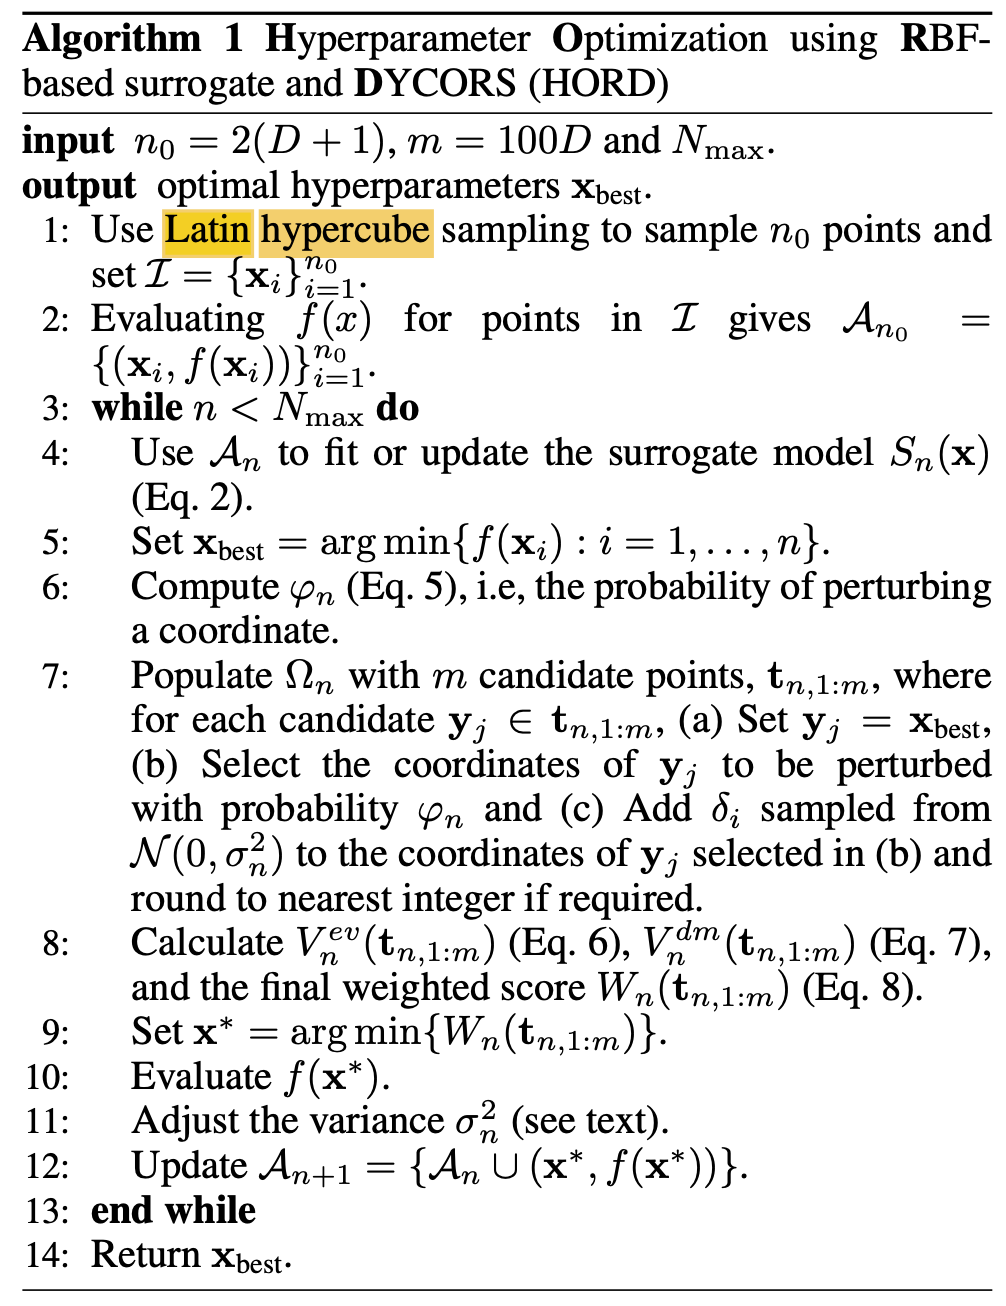
\includegraphics[width=0.5\textwidth]{pseudocode.png}
  \end{figure}
\end{frame}


\begin{frame}
  \frametitle{Experimental setup}
  \textbf{Experiments}
  \begin{enumerate}
    \item \textbf{6-MLP}: 4 continuous and 2 integer hyperparameters.
    \item \textbf{8-CNN}: 4 continuous and 4 integer hyperparameters.
    \item \textbf{15-CNN}: 10 continuous and 5 integer hyperparameters.
    \item \textbf{19-CNN}: 14 continuous and 5 integer hyperparameters.
  \end{enumerate}
  \textbf{Baselines}
  \begin{enumerate}
    \item \textbf{GP-EI}: Gaussian processes with expected improvemen.
    \item \textbf{GP-PES}: Gaussian processes with predictive entropy search
    \item \textbf{TPE}: Tree Parzen Estimator
    \item \textbf{SMAC}: Sequential Model-based Algorithm Configuration
  \end{enumerate}
\end{frame}


\begin{frame}
  \frametitle{Experimental Results}
  \begin{figure}
    \hfill
    \subfigure[Speed comparison.]{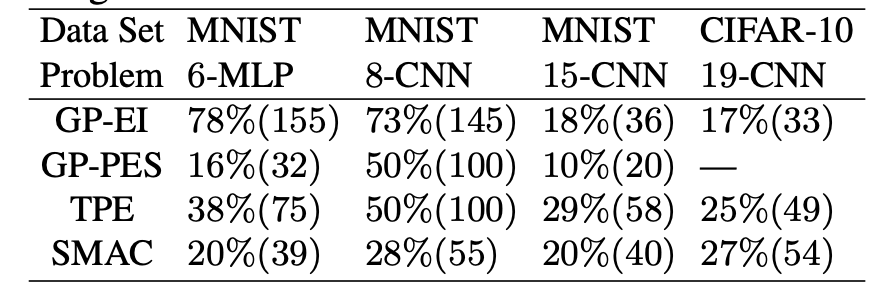
\includegraphics[width=0.45\textwidth]{speed.png}}
    \hfill
    \subfigure[Test error comparison.]{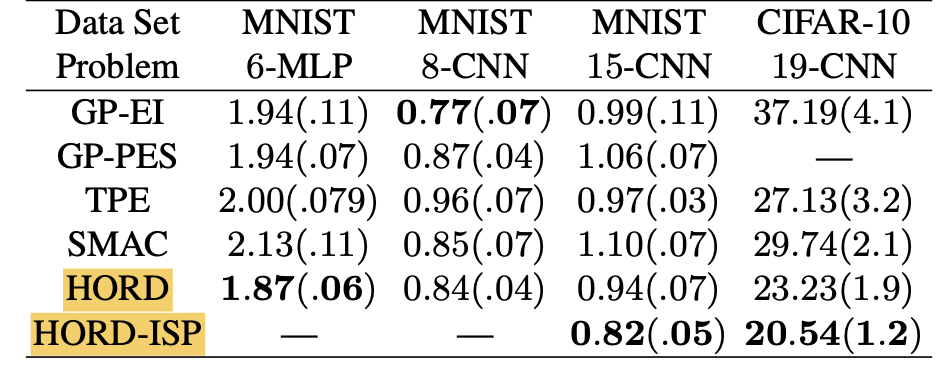
\includegraphics[width=0.45\textwidth]{quality.png}}
    \hfill
    \end{figure}
    We see that HORD (HORD-ISP) outperforms the baselines in terms of accuracy and speed.
\end{frame}


\begin{frame}
  \frametitle{References}
  \begin{thebibliography}{9}
    % \bibitem{texbook}
    % Donald E. Knuth (1986) \emph{The \TeX{} Book}, Addison-Wesley Professional.
    
    % \bibitem{lamport94}
    % Leslie Lamport (1994) \emph{\LaTeX: a document preparation system}, Addison
    % Wesley, Massachusetts, 2nd ed.
    \bibitem{rbf}
    Gutmann H. M. (2001) A radial basis function method for global optimization, Journal of global optimization.

    \bibitem{textbook}
    https://artowen.su.domains/mc/Ch-var-adv.pdf

    \bibitem{paper}
    Ilievski I. et al. (2017) Efficient hyperparameter optimization for deep learning algorithms using deterministic rbf surrogates, Proceedings of the AAAI conference on artificial intelligence.
    \end{thebibliography}
  
\end{frame}



\end{document}